% Copyright 2018 Melvin Eloy Irizarry-Gelpí
\chapter{Motion on an Incline}
%%%%%%%%%%%%%%%%%%%%%%%%%%%%%%%%%%%%%%%%%%%%%%%%%%%%%%%%%%%%%%%%%%%%%%%%%%%%%%%%
In this experiment you will study motion on an incline plane and confirm that the mathematical descriptions introduced in class for motion with constant acceleration also applies to this case.
%%%%%%%%%%%%%%%%%%%%%%%%%%%%%%%%%%%%%%%%%%%%%%%%%%%%%%%%%%%%%%%%%%%%%%%%%%%%%%%%
\section{Preliminary}
%%%%%%%%%%%%%%%%%%%%%%%%%%%%%%%%%%%%%%%%%%%%%%%%%%%%%%%%%%%%%%%%%%%%%%%%%%%%%%%%
If you ignore the effects of air resistance, the acceleration of an object that falls freely is constant. Since \textbf{acceleration} is the \textbf{rate of change of velocity with time}, this means that the rate of change of velocity with time is constant. If a dependent variable $v$ has a constant rate of change with respect to an independent variable $t$, then there is a mathematical relation of the form
\begin{equation}
    v = m t + b
    \label{eq:02.v.linear}
\end{equation}
This relation describes a \textbf{linear shape}. In the previous experiment you learned that, for free-fall, the slope $m$ corresponds to the acceleration due to gravity $g$, and the intercept $b$ corresponds to the initial (vertical) velocity $v_{0}$. That is,
\begin{equation}
    v = g t + v_{0}
\end{equation}
If the acceleration is a different constant value $a$, then you just replace $g$ with $a$.

\textbf{Velocity} is the \textbf{rate of change of position with time}. If the velocity depends on time in a linear way (i.e. as in Equation \ref{eq:02.v.linear}), then the spatial position $d$ (distance to a fixed point) and time $t$ will obey a mathematical relation of the form
\begin{equation}
    d = A t^{2} + B t + C
    \label{eq:02.d.quadratic}
\end{equation}
This relation describes a \textbf{parabolic shape}. Here, $A$ must be a quantity with units of acceleration, $B$ must be a quantity with units of velocity, and $C$ must be a quantity with units of distance. Indeed, $A$ in Equation \ref{eq:02.d.quadratic} must be related to the slope $m$ in Equation \ref{eq:02.v.linear} via
\begin{equation}
    A = \frac{1}{2} m
\end{equation}
and $B$ in Equation \ref{eq:02.d.quadratic} must be related to the intercept $b$ in Equation \ref{eq:02.v.linear} via
\begin{equation}
    B = b
\end{equation}
That is, the parameters determining $d$ in Equation \ref{eq:02.d.quadratic} determine the parameters in Equation \ref{eq:02.v.linear}. The interpretation of $C$ in Equation \ref{eq:02.d.quadratic} is as the value that $d$ takes when $t = 0$ (the initial distance).

Motion with \textbf{constant acceleration} is not only restricted to free-fall. As you will observe from the data, it also describes motion along an inclined track. However, the value of the constant acceleration is not the acceleration due to gravity, but a fraction of it.
%%%%%%%%%%%%%%%%%%%%%%%%%%%%%%%%%%%%%%%%%%%%%%%%%%%%%%%%%%%%%%%%%%%%%%%%%%%%%%%%
\section{Experiment}
%%%%%%%%%%%%%%%%%%%%%%%%%%%%%%%%%%%%%%%%%%%%%%%%%%%%%%%%%%%%%%%%%%%%%%%%%%%%%%%%
You used a motion sensor to measure the position, velocity, and acceleration of a cart traveling along an inclined track. You also recorded the height of certain points along the incline.
%%%%%%%%%%%%%%%%%%%%%%%%%%%%%%%%%%%%%%%%%%%%%%%%%%%%%%%%%%%%%%%%%%%%%%%%%%%%%%%%
\section{Analysis}
%%%%%%%%%%%%%%%%%%%%%%%%%%%%%%%%%%%%%%%%%%%%%%%%%%%%%%%%%%%%%%%%%%%%%%%%%%%%%%%%
The goal is to describe the motion along the inclined track. Preliminary observations suggest constant acceleration. In order to confirm this, you should check that the behavior of position, velocity, and acceleration are consistent. Here are the steps to follow.
%%%%%%%%%%%%%%%%%%%%%%%%%%%%%%%%%%%%%%%%%%%%%%%%%%%%%%%%%%%%%%%%%%%%%%%%%%%%%%%%
\subsection{Find the Sine of the Angles of Inclination}
%%%%%%%%%%%%%%%%%%%%%%%%%%%%%%%%%%%%%%%%%%%%%%%%%%%%%%%%%%%%%%%%%%%%%%%%%%%%%%%%
The inclined track is characterized by the \textbf{angle of inclination}. The larger the angle, the more inclined the track is. You do not need to find the actual angle, only the \textbf{sine of the angle} (sine as in trigonometry). Here is how to find that sine for each of the two cases (one-box height and two-box height).
%%%%%%%%%%%%%%%%%%%%%%%%%%%%%%%%%%%%%%%%%%%%%%%%%%%%%%%%%%%%%%%%%%%%%%%%%%%%%%%%
\subsubsection{Measure the heights of points along incline}
%%%%%%%%%%%%%%%%%%%%%%%%%%%%%%%%%%%%%%%%%%%%%%%%%%%%%%%%%%%%%%%%%%%%%%%%%%%%%%%%
You choose about \textbf{four points along the incline} and use a ruler to measure the vertical distance from the top of the incline to the surface of the table. In Table \ref{table:02.height.2} and Table \ref{table:02.height.1} you can find my measurements for the two-box and one-box cases.
%%%%%%%%%%%%%%%%%%%%%%%%%%%%%%%%%%%%%%%%%%%%%%%%%%%%%%%%%%%%%%%%%%%%%%%%%%%%%%%%
\subsubsection{Calculate the differences in position}
%%%%%%%%%%%%%%%%%%%%%%%%%%%%%%%%%%%%%%%%%%%%%%%%%%%%%%%%%%%%%%%%%%%%%%%%%%%%%%%%
You can take distinct positions and calculate the differences. For example, consider the two-box case and the first two measurements (label 1 and 2) in Table \ref{table:02.height.2}. The first two heights are $h_{1} = 8.9$ cm and $h_{2} = 11.7$ cm. The \textbf{difference} is
\begin{equation}
    \Delta h = h_{2} - h_{1} = 2.8 \text{ cm}
\end{equation}
Similarly, the first two positions along the incline are $d_{1} = 25$ cm and $d_{2} = 50$ cm. The \textbf{difference} is
\begin{equation}
    \Delta d = d_{2} - d_{1} = 25 \text{ cm}
\end{equation}
If you have \textbf{four} pairs of positions (as in Table \ref{table:02.height.2} and Table \ref{table:02.height.1}), then you should be able to calculate \textbf{six} distinct differences for each dimension. In Table \ref{table:02.sine.2} and Table \ref{table:02.sine.1} you can find the values of my differences.
%%%%%%%%%%%%%%%%%%%%%%%%%%%%%%%%%%%%%%%%%%%%%%%%%%%%%%%%%%%%%%%%%%%%%%%%%%%%%%%%
\subsubsection{Calculate the ratios of differences to find sine}
%%%%%%%%%%%%%%%%%%%%%%%%%%%%%%%%%%%%%%%%%%%%%%%%%%%%%%%%%%%%%%%%%%%%%%%%%%%%%%%%
The sine of the angle of inclination is given by the ratio of differences:
\begin{equation}
    \sin(\theta) = \frac{\Delta h}{\Delta d}
\end{equation}
For each pair of differences $\Delta h$ and $\Delta d$, you can calculate a value of this ratio. Using the differences mentioned above for the two-box case, the sine is
\begin{equation}
    \sin(\theta) = \frac{2.8 \text{ cm}}{25 \text{ cm}} = 0.112
\end{equation}
The sine values for the one-box and two-box cases are in Table \ref{table:02.sine.2} and Table \ref{table:02.sine.1}. Since the two boxes that you used to raise the track are almost the same height, it follows that the sine for the two-box case should be almost twice the value of the sine for the one-box case.
%%%%%%%%%%%%%%%%%%%%%%%%%%%%%%%%%%%%%%%%%%%%%%%%%%%%%%%%%%%%%%%%%%%%%%%%%%%%%%%%
\subsection{Fit Position Data}
%%%%%%%%%%%%%%%%%%%%%%%%%%%%%%%%%%%%%%%%%%%%%%%%%%%%%%%%%%%%%%%%%%%%%%%%%%%%%%%%
You can plot the \textbf{position column versus the time column}. One of my runs is in Figure \ref{figure:02.raw.d}. As you can see, there is a region that looks like a parabola. Before attempting to fit the data, you need to truncate the part of the data before and after the parabola. This step is highly subjective: it depends on your judgement. Note that the parabola begins to smoothly ramp-up: I chose to not include this ramping-up and instead decided to cut the parabola around just when the position is close to 0.2 m.

After isolating the parabola segment, you can add the best fit curve. Instead of using a linear fit, you need to use a \textbf{polynomial fit}. First, go to
\begin{equation}
    \texttt{Chart editor > CUSTOMIZE > Series}
\end{equation}
and check on \texttt{Trendline}. Then,
\begin{itemize}
    \item Under \texttt{Type} select \texttt{Polynomial}.
    \item Under \texttt{Line color} change from blue to red or something else that is easier to distinguish from the data.
    \item Make sure that under \texttt{Polynomial Degree} the value is \texttt{2}.
    \item Finally, under \texttt{Label} select \texttt{Use Equation}.
\end{itemize}
You should see the legend with the data and the equation for the best-fit quadratic function of the form:
\begin{equation}
    \texttt{CCC + BBBx + AAAx\^{}2}
\end{equation}
The value in \texttt{CCC} corresponds to $C$ in Equation \ref{eq:02.d.quadratic}; the value in \texttt{BBB} corresponds to $B$; and the value in \texttt{AAA} corresponds to $A$.

After deleting the non-parabolic segments, the best-fit parabola should be very close to the data. Figure \ref{figure:02.fit.d} shows one of my runs with the fit.
%%%%%%%%%%%%%%%%%%%%%%%%%%%%%%%%%%%%%%%%%%%%%%%%%%%%%%%%%%%%%%%%%%%%%%%%%%%%%%%%
\subsection{Fit Velocity Data}
%%%%%%%%%%%%%%%%%%%%%%%%%%%%%%%%%%%%%%%%%%%%%%%%%%%%%%%%%%%%%%%%%%%%%%%%%%%%%%%%
You can plot the \textbf{velocity column versus the time column}. One of my runs is in Figure \ref{figure:02.raw.v}. As you can see, there is a region that looks like a diagonal line. Just like for the position data, before attempting to fit the data you need to truncate the non-linear parts.

For the position data, when you delete the non-parabolic region, you can also delete the corresponding velocity values. Once you have restricted to a subset that keeps the parabolic segment only, you can look at the velocity data inside this same time segment. The linear fit should now be appropriate. Figure \ref{figure:02.fit.v} shows one of my runs with the fit.
%%%%%%%%%%%%%%%%%%%%%%%%%%%%%%%%%%%%%%%%%%%%%%%%%%%%%%%%%%%%%%%%%%%%%%%%%%%%%%%%
\subsection{Average Acceleration Data}
%%%%%%%%%%%%%%%%%%%%%%%%%%%%%%%%%%%%%%%%%%%%%%%%%%%%%%%%%%%%%%%%%%%%%%%%%%%%%%%%
You can plot the \textbf{acceleration column versus the time column}. One of my runs is in Figure \ref{figure:02.raw.a}. As you can see, there is a region that looks like a horizontal flat line. This would indicate a segment where the acceleration takes a constant value. But just like for the position and velocity data, before you can estimate the value of the constant you need to truncate the non-flat parts.

You can remove the acceleration values that occur at the same times that you removed in order to get rid of the non-parabolic parts for the position data. Once you have restricted to that subset, you might still observe regions that are not part of the flat segment. Still, for simplicity, you can keep them.

Due to noise and computational errors, the flat segment is not truly flat. One way to estimate the value of the constant acceleration is to calculate the average. Figure \ref{figure:02.fit.a} shows one of my runs with the flat line corresponding to the average acceleration. 
%%%%%%%%%%%%%%%%%%%%%%%%%%%%%%%%%%%%%%%%%%%%%%%%%%%%%%%%%%%%%%%%%%%%%%%%%%%%%%%%
\subsection{Confirm Constant Acceleration Model}
%%%%%%%%%%%%%%%%%%%%%%%%%%%%%%%%%%%%%%%%%%%%%%%%%%%%%%%%%%%%%%%%%%%%%%%%%%%%%%%%
There are many checks you can do to confirm that the data corresponds to motion with constant acceleration.
%%%%%%%%%%%%%%%%%%%%%%%%%%%%%%%%%%%%%%%%%%%%%%%%%%%%%%%%%%%%%%%%%%%%%%%%%%%%%%%%
\subsubsection{Check consistency of acceleration}
%%%%%%%%%%%%%%%%%%%%%%%%%%%%%%%%%%%%%%%%%%%%%%%%%%%%%%%%%%%%%%%%%%%%%%%%%%%%%%%%
This check involves comparing the values of
\begin{enumerate}
    \item $2A$ with $A$ the quadratic coefficient in the position fit,
    \item the value of the slope in the velocity fit,
    \item and the average value from the acceleration data.
\end{enumerate}
These three values should be close, and should be the same across the three runs with the same height. You can see my results in Table \ref{table:02.check.a}.
%%%%%%%%%%%%%%%%%%%%%%%%%%%%%%%%%%%%%%%%%%%%%%%%%%%%%%%%%%%%%%%%%%%%%%%%%%%%%%%%
\subsubsection{Check agreement $g$}
%%%%%%%%%%%%%%%%%%%%%%%%%%%%%%%%%%%%%%%%%%%%%%%%%%%%%%%%%%%%%%%%%%%%%%%%%%%%%%%%
The specific value of the constant acceleration should be a particular fraction of the acceleration due to gravity. Namely,
\begin{equation}
    a = g \sin(\theta)
\end{equation}
Equivalently, you can flip this equation and use it to estimate the value of $g$:
\begin{equation}
    g = \frac{a}{\sin(\theta)}
\end{equation}
Since you have three estimates for the acceleration (see previous check), for each run, you can calculate three estimates for the acceleration due to gravity. The results should be close to the accepted value of 9.80 m/s$^{2}$. You can see my results in Table \ref{table:02.check.g}.
%%%%%%%%%%%%%%%%%%%%%%%%%%%%%%%%%%%%%%%%%%%%%%%%%%%%%%%%%%%%%%%%%%%%%%%%%%%%%%%%
\subsubsection{Check consistency of initial velocity}
%%%%%%%%%%%%%%%%%%%%%%%%%%%%%%%%%%%%%%%%%%%%%%%%%%%%%%%%%%%%%%%%%%%%%%%%%%%%%%%%
The initial velocity should be consistent also. That is, compare the values of
\begin{enumerate}
    \item $B$ the linear coefficient in the position fit,
    \item and the value of the intercept in the velocity fit.
\end{enumerate}
The specific value will be different for every run (it depends on how you launched the cart), but for a given run, the two values should be close. You can see my results in Table \ref{table:02.check.v0}.
%%%%%%%%%%%%%%%%%%%%%%%%%%%%%%%%%%%%%%%%%%%%%%%%%%%%%%%%%%%%%%%%%%%%%%%%%%%%%%%%
\section{My Data}
%%%%%%%%%%%%%%%%%%%%%%%%%%%%%%%%%%%%%%%%%%%%%%%%%%%%%%%%%%%%%%%%%%%%%%%%%%%%%%%%
My data consist of six runs:
\begin{itemize}
    \item Runs 1, 2, 3: two-box case
    \item Runs 4, 5, 6: one-box case
\end{itemize}
Each run is about 5 seconds long.
%%%%%%%%%%%%%%%%%%%%%%%%%%%%%%%%%%%%%%%%%%%%%%%%%%%%%%%%%%%%%%%%%%%%%%%%%%%%%%%%
\section{Your Data}
%%%%%%%%%%%%%%%%%%%%%%%%%%%%%%%%%%%%%%%%%%%%%%%%%%%%%%%%%%%%%%%%%%%%%%%%%%%%%%%%
You should have six runs with three for the one-box case, and three for the two-box case. Make sure that you do not get them mixed up!
%%%%%%%%%%%%%%%%%%%%%%%%%%%%%%%%%%%%%%%%%%%%%%%%%%%%%%%%%%%%%%%%%%%%%%%%%%%%%%%%
\section{Your Laboratory Report}
%%%%%%%%%%%%%%%%%%%%%%%%%%%%%%%%%%%%%%%%%%%%%%%%%%%%%%%%%%%%%%%%%%%%%%%%%%%%%%%%
Your laboratory report should include the following:
\begin{enumerate}
    \item \textbf{One} chart with \textbf{position} in the vertical axis, and \textbf{time} in the horizontal axis, showing the \textbf{full time interval} (see Figure \ref{figure:02.raw.d}). Label the region in the chart where the cart is moving up the ramp, stopped, and moving down the ramp.
    \item \textbf{One} chart with \textbf{position} in the vertical axis, and \textbf{time} in the horizontal axis, showing the \textbf{parabolic segment only}. Include the best-fit quadratic function and make sure you display the equation in the legend (see Figure \ref{figure:02.fit.d}). 
    \item \textbf{One} chart with \textbf{velocity} in the vertical axis, and \textbf{time} in the horizontal axis, showing the \textbf{full time interval} (see Figure \ref{figure:02.raw.v}). Label the region in the chart where the cart is moving up the ramp, stopped, and moving down the ramp.
    \item \textbf{One} chart with \textbf{velocity} in the vertical axis, and \textbf{time} in the horizontal axis, showing the \textbf{linear segment only}. Include the best-fit linear function and make sure you display the equation in the legend (see Figure \ref{figure:02.fit.v}).
    \item \textbf{One} chart with \textbf{acceleration} in the vertical axis, and \textbf{time} in the horizontal axis, showing the \textbf{full time interval} (see Figure \ref{figure:02.raw.a}). Label the region in the chart where the cart is moving up the ramp, stopped, and moving down the ramp.
\end{enumerate}
You are free to choose which run to use for each chart. However, in order to obtain the quadratic fit parameters, you need to produce all charts in your spreadsheet. You should also include the following:
\begin{enumerate}
    \item Tables like Table \ref{table:02.height.2} and Table \ref{table:02.height.1} with your four height measurements.
    \item Tables like Table \ref{table:02.sine.2} and Table \ref{table:02.sine.1} with the sine values for both the one-box and two-box cases.
    \item Tables like Table \ref{table:02.fit.d}, Table \ref{table:02.fit.v}, and Table \ref{table:02.fit.a} with the values obtained from fitting or averaging.
    \item Tables like Table \ref{table:02.check.a}, Table \ref{table:02.check.g}, and Table \ref{table:02.check.v0} with checks for constancy of the acceleration.
\end{enumerate}
%%%%%%%%%%%%%%%%%%%%%%%%%%%%%%%%%%%%%%%%%%%%%%%%%%%%%%%%%%%%%%%%%%%%%%%%%%%%%%%%
\newpage
\section{Tables}
%%%%%%%%%%%%%%%%%%%%%%%%%%%%%%%%%%%%%%%%%%%%%%%%%%%%%%%%%%%%%%%%%%%%%%%%%%%%%%%%
\begin{table}[ht]
    \centering
    \begin{tabular}{|l|r|r|}
        \hline
        \textbf{Label} & $d$ (cm) & $h$ (cm) \\
        \hline
        1 & 25 & 8.9 \\
        2 & 50 & 11.7 \\
        3 & 75 & 14.6 \\
        4 & 100 & 17.5 \\
        \hline
    \end{tabular}
    \caption{Position along incline and height for \textbf{two-box} case}
    \label{table:02.height.2}
\end{table}
%%%%%%%%%%%%%%%%%%%%%%%%%%%%%%%%%%%%%%%%%%%%%%%%%%%%%%%%%%%%%%%%%%%%%%%%%%%%%%%%
\begin{table}[ht]
    \centering
    \begin{tabular}{|l|r|r|}
        \hline
        \textbf{Label} & $d$ (cm) & $h$ (cm) \\
        \hline
        1 & 25 & 8.2 \\
        2 & 50 & 9.4 \\
        3 & 75 & 10.8 \\
        4 & 100 & 12.3 \\
        \hline
    \end{tabular}
    \caption{Position along incline and height for \textbf{one-box} case}
    \label{table:02.height.1}
\end{table}
%%%%%%%%%%%%%%%%%%%%%%%%%%%%%%%%%%%%%%%%%%%%%%%%%%%%%%%%%%%%%%%%%%%%%%%%%%%%%%%%
\begin{table}[ht]
    \centering
    \begin{tabular}{|l|r|r|r|}
        \hline
        \textbf{Labels} & $\Delta d$ (cm) & $\Delta h$ (cm) & $\sin(\theta) = \Delta h / \Delta d$ \\
        \hline
        2 and 1 & 25 & 2.8 & 0.112 \\
        3 and 2 & 25 & 2.9 & 0.116 \\
        3 and 1 & 50 & 5.7 & 0.114 \\
        4 and 3 & 25 & 2.9 & 0.116 \\
        4 and 2 & 50 & 5.8 & 0.116 \\
        4 and 1 & 75 & 8.6 & 0.115 \\
        \hline
    \end{tabular}
    \caption{Sine for angle of inclination for \textbf{two-box} case. Average is 0.115.}
    \label{table:02.sine.2}
\end{table}
%%%%%%%%%%%%%%%%%%%%%%%%%%%%%%%%%%%%%%%%%%%%%%%%%%%%%%%%%%%%%%%%%%%%%%%%%%%%%%%%
\begin{table}[ht]
    \centering
    \begin{tabular}{|l|r|r|r|}
        \hline
        \textbf{Labels} & $\Delta d$ (cm) & $\Delta h$ (cm) & $\sin(\theta) = \Delta h / \Delta d$ \\
        \hline
        2 and 1 & 25 & 1.2 & 0.048 \\
        3 and 2 & 25 & 1.4 & 0.056 \\
        3 and 1 & 50 & 2.6 & 0.052 \\
        4 and 3 & 25 & 1.5 & 0.060 \\
        4 and 2 & 50 & 2.9 & 0.058 \\
        4 and 1 & 75 & 4.1 & 0.055 \\
        \hline
    \end{tabular}
    \caption{Sine for angle of inclination for \textbf{one-box} case. Average is 0.055.}
    \label{table:02.sine.1}
\end{table}
%%%%%%%%%%%%%%%%%%%%%%%%%%%%%%%%%%%%%%%%%%%%%%%%%%%%%%%%%%%%%%%%%%%%%%%%%%%%%%%%
\begin{table}[ht]
    \centering
    \begin{tabular}{|l|r|r|r|}
        \hline
        \textbf{Run} & $C$ (m) & $B$ (m/s) & $A$ (m/s$^{2}$) \\
        \hline
        1 & -1.29 & 2.14 & -0.557 \\
        2 & -1.07 & 1.95 & -0.551 \\
        3 & -0.955 & 1.94 & -0.552 \\
        \hline
        4 & -1.58 & 1.53 & -0.26 \\
        5 & -0.749 & 1.28 & -0.26 \\
        6 & -1.23 & 1.48 & -0.261 \\
        \hline
    \end{tabular}
    \caption{Summary of results: fit parameters from \textbf{position} data}
    \label{table:02.fit.d}
\end{table}
%%%%%%%%%%%%%%%%%%%%%%%%%%%%%%%%%%%%%%%%%%%%%%%%%%%%%%%%%%%%%%%%%%%%%%%%%%%%%%%%
\begin{table}[ht]
    \centering
    \begin{tabular}{|l|r|r|}
        \hline
        \textbf{Run} & \textbf{Slope} (m/s$^{2}$) & \textbf{Intercept} (m/s) \\
        \hline
        1 & -1.13 & 2.16 \\
        2 & -1.09 & 1.94 \\
        3 & -1.08 & 1.9 \\
        \hline
        4 & -0.519 & 1.53 \\
        5 & -0.516 & 1.28 \\
        6 & -0.52 & 1.48 \\
        \hline
    \end{tabular}
    \caption{Summary of results: fit parameters from \textbf{velocity} data}
    \label{table:02.fit.v}
\end{table}
%%%%%%%%%%%%%%%%%%%%%%%%%%%%%%%%%%%%%%%%%%%%%%%%%%%%%%%%%%%%%%%%%%%%%%%%%%%%%%%%
\begin{table}[ht]
    \centering
    \begin{tabular}{|l|r|}
        \hline
        \textbf{Run} & \textbf{Average Acceleration} (m/s$^{2}$) \\
        \hline
        1 & -1.030 \\
        2 & -1.010 \\
        3 & -1.054 \\
        \hline
        4 & -0.514 \\
        5 & -0.488 \\
        6 & -0.494 \\
        \hline
    \end{tabular}
    \caption{Summary of results: average \textbf{acceleration}}
    \label{table:02.fit.a}
\end{table}
%%%%%%%%%%%%%%%%%%%%%%%%%%%%%%%%%%%%%%%%%%%%%%%%%%%%%%%%%%%%%%%%%%%%%%%%%%%%%%%%
\begin{table}[ht]
    \centering
    \begin{tabular}{|l|r|r|r|r|}
        \hline
        \textbf{Run} & $A$ & $2A$ & \textbf{Slope} & \textbf{Average Acceleration} \\
        \hline
        1 & -0.557 & -1.114 & -1.13 & -1.030 \\
        2 & -0.551 & -1.102 & -1.09 & -1.010 \\
        3 & -0.552 & -1.104 & -1.08 & -1.054 \\
        \hline
        4 & -0.26 & -0.52 & -0.519 & -0.514 \\
        5 & -0.26 & -0.52 & -0.516 & -0.488 \\
        6 & -0.261 & -0.522 & -0.52 & -0.494 \\
        \hline
    \end{tabular}
    \caption{Checks for constant acceleration: consistent acceleration across measurements. All values in the last four columns are in units of m/s$^{2}$.}
    \label{table:02.check.a}
\end{table}
%%%%%%%%%%%%%%%%%%%%%%%%%%%%%%%%%%%%%%%%%%%%%%%%%%%%%%%%%%%%%%%%%%%%%%%%%%%%%%%%
\begin{table}[ht]
    \centering
    \begin{tabular}{|l|r|r|r|r|}
        \hline
        \textbf{Run} & $\sin(\theta)$ & $2A / \sin(\theta)$ & $\text{Slope}/\sin(\theta)$ & $(\text{Average Acceleration})/\sin(\theta)$ \\
        \hline
        1 & 0.115 & -9.706 & -9.845 & -8.974 \\
        2 & 0.115 & -9.601 & -9.497 & -8.796 \\
        3 & 0.115 & -9.619 & -9.409 & -9.180 \\
        \hline
        4 & 0.055 & -9.493 & -9.475 & -9.383 \\
        5 & 0.055 & -9.493 & -9.420 & -8.909 \\
        6 & 0.055 & -9.529 & -9.493 & -9.018 \\
        \hline
    \end{tabular}
    \caption{Checks for constant acceleration: agreement with $g = -9.80$ m/s$^{2}$. All values in the last three columns are in units of m/s$^{2}$.}
    \label{table:02.check.g}
\end{table}
%%%%%%%%%%%%%%%%%%%%%%%%%%%%%%%%%%%%%%%%%%%%%%%%%%%%%%%%%%%%%%%%%%%%%%%%%%%%%%%%
\begin{table}[ht]
    \centering
    \begin{tabular}{|l|r|r|}
        \hline
        \textbf{Run} & $B$ (m/s) & \textbf{Intercept} (m/s) \\
        \hline
        1 & 2.14 & 2.16 \\
        2 & 1.95 & 1.94 \\
        3 & 1.94 & 1.9 \\
        \hline
        4 & 1.53 & 1.53 \\
        5 & 1.28 & 1.28 \\
        6 & 1.48 & 1.48 \\
        \hline
    \end{tabular}
    \caption{Checks for constant acceleration: comparing intercept and $B$.}
    \label{table:02.check.v0}
\end{table}
%%%%%%%%%%%%%%%%%%%%%%%%%%%%%%%%%%%%%%%%%%%%%%%%%%%%%%%%%%%%%%%%%%%%%%%%%%%%%%%%
\FloatBarrier
\newpage
\section{Figures}
%%%%%%%%%%%%%%%%%%%%%%%%%%%%%%%%%%%%%%%%%%%%%%%%%%%%%%%%%%%%%%%%%%%%%%%%%%%%%%%%
\begin{figure}[ht]
    \centering
    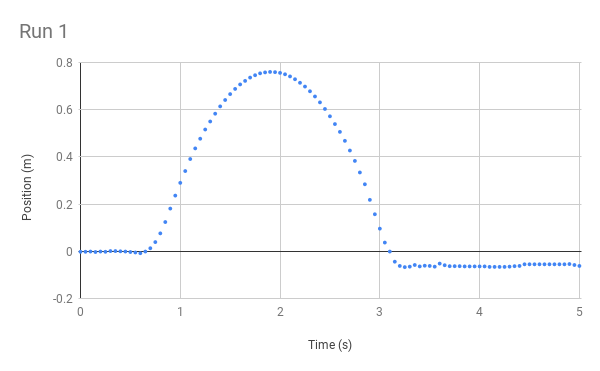
\includegraphics[scale=0.71]{image/02-incline/Run1-d.png}
    \caption{Full raw position data for run 1}
    \label{figure:02.raw.d}
\end{figure}
%%%%%%%%%%%%%%%%%%%%%%%%%%%%%%%%%%%%%%%%%%%%%%%%%%%%%%%%%%%%%%%%%%%%%%%%%%%%%%%%
\begin{figure}[ht]
    \centering
    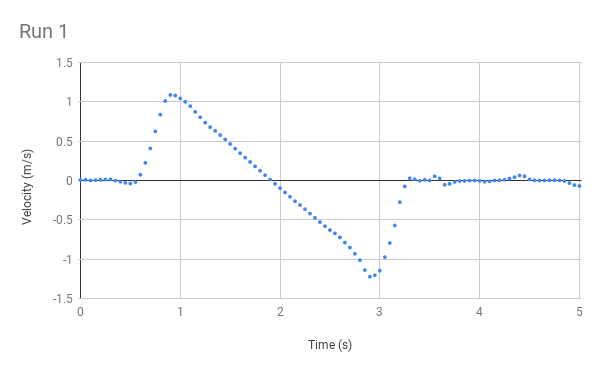
\includegraphics[scale=0.71]{image/02-incline/Run1-v.png}
    \caption{Full raw velocity data for run 1}
    \label{figure:02.raw.v}
\end{figure}
%%%%%%%%%%%%%%%%%%%%%%%%%%%%%%%%%%%%%%%%%%%%%%%%%%%%%%%%%%%%%%%%%%%%%%%%%%%%%%%%
\begin{figure}[ht]
    \centering
    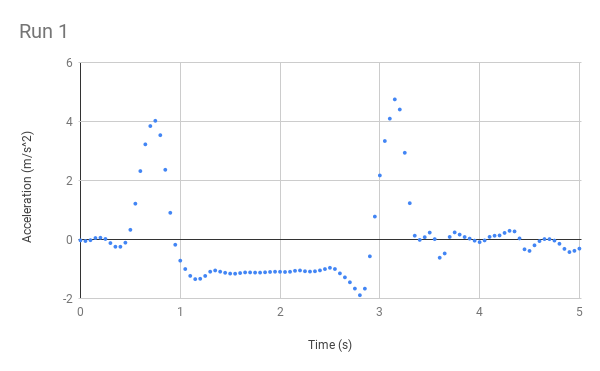
\includegraphics[scale=0.71]{image/02-incline/Run1-a.png}
    \caption{Full raw acceleration data for run 1}
    \label{figure:02.raw.a}
\end{figure}
%%%%%%%%%%%%%%%%%%%%%%%%%%%%%%%%%%%%%%%%%%%%%%%%%%%%%%%%%%%%%%%%%%%%%%%%%%%%%%%%
\begin{figure}[ht]
    \centering
    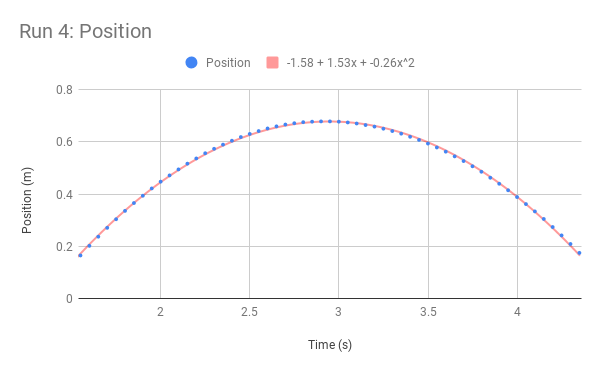
\includegraphics[scale=0.71]{image/02-incline/Run-4-d.png}
    \caption{Quadratic fit of position data for run 4}
    \label{figure:02.fit.d}
\end{figure}
%%%%%%%%%%%%%%%%%%%%%%%%%%%%%%%%%%%%%%%%%%%%%%%%%%%%%%%%%%%%%%%%%%%%%%%%%%%%%%%%
\begin{figure}[ht]
    \centering
    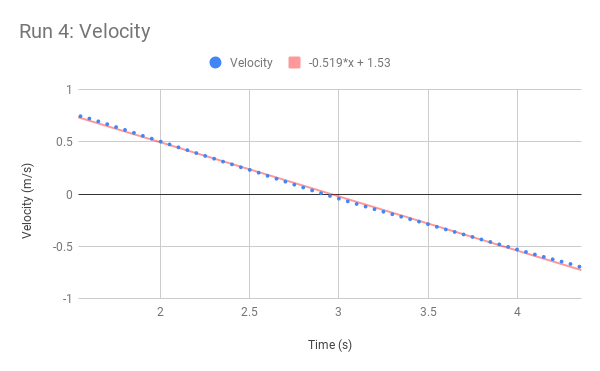
\includegraphics[scale=0.71]{image/02-incline/Run-4-v.png}
    \caption{Linear fit of velocity data for run 4}
    \label{figure:02.fit.v}
\end{figure}
%%%%%%%%%%%%%%%%%%%%%%%%%%%%%%%%%%%%%%%%%%%%%%%%%%%%%%%%%%%%%%%%%%%%%%%%%%%%%%%%
\begin{figure}[ht]
    \centering
    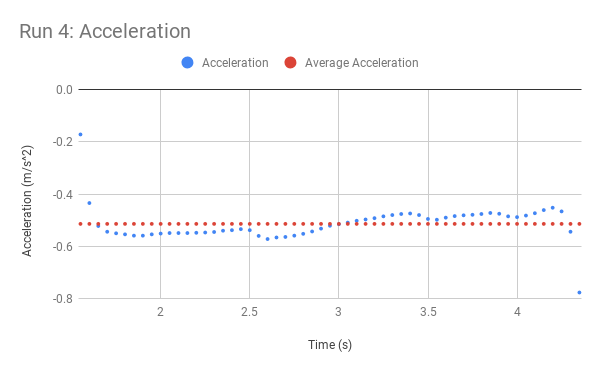
\includegraphics[scale=0.71]{image/02-incline/Run-4-a.png}
    \caption{Average value for acceleration data for run 4}
    \label{figure:02.fit.a}
\end{figure}
%%%%%%%%%%%%%%%%%%%%%%%%%%%%%%%%%%%%%%%%%%%%%%%%%%%%%%%%%%%%%%%%%%%%%%%%%%%%%%%%